\documentclass[amsfonts, amssymb, prl, superscriptaddress, notitlepage, twocolumn, nofootinbib]{revtex4-2}

\usepackage{amsmath}    
\usepackage{graphicx}   
\usepackage{verbatim}   
\usepackage{color}      
\usepackage{hyperref}   
%\usepackage{subcaption}
\usepackage[english]{babel}
\usepackage{ucs}
\usepackage[utf8x]{inputenc}
\usepackage{subfigure}
\usepackage[autostyle]{csquotes}
%\MakeOuterQuote{"}
\usepackage{float}
\usepackage{textcomp}
\usepackage{xspace}
\usepackage{orcidlink}



\newcommand{\Corr}{\operatorname{Corr}}
\newcommand{\Cov}{\operatorname{Cov}}
\DeclareMathOperator{\E}{\mathbb{E}} 
\DeclareMathOperator{\Var}{Var}
\newcommand{\bc}[2]{$\beta$#1cell#2}
\newcommand{\lra}[1]{\langle{}#1\rangle}
\newcommand{\Ca}{Ca$^{2+}$\xspace}
\newcommand{\Cac}{[Ca${}^{2+}$]$_{\rm{c}}$\xspace}


\begin{document}

\title{Two cultures}
\author{L.~Kopitar \orcidlink{0000-0002-6647-9988}}
\affiliation{University of Maribor, Faculty of Health Sciences, Slovenia}

\author{N.~Plohl}
\affiliation{University of Maribor, Faculty of Arts, Slovenia}

\author{M.~Tancer Verboten}
\affiliation{University of Maribor, Faculty of Law, Slovenia}
\affiliation{University of Maribor, Faculty of Chemistry and Chemical Engineering, Slovenia}


\author{G.~Štiglic \orcidlink{0000-0002-0183-8679}}
\affiliation{University of Maribor, Faculty of Health Sciences, Slovenia}

\author{R.~Watson \orcidlink{0000-0001-8040-7625}}
\affiliation{Southwest Medical University, China }

\author{D.~Korošak \orcidlink{0000-0003-3818-1233} }
\thanks{Corresponding author:\\dean.korosak@um.si}
\affiliation{University of Maribor, Faculty of Medicine, Slovenia}
\affiliation{University of Maribor, Faculty of Civil Engineering, Transportation Engineering and Architecture, Maribor, Slovenia}
% https://orcid.org/0000-0003-3818-1233




\date{\today}

\begin{abstract}
Results showed significant differences in publishing practices, with a clear and robust separation of EU countries into two groups with distinct scholarly publishing cultures.
\end{abstract}

\maketitle 

\section{Introduction}
One of the mainstays of evaluating the performance of universities is their performance in research, and a major plank of that evaluation is constituted by publication in academic journals. Likewise, the evaluation of individual academics follows similar processes. 
We have previously discussed the controversies involved in using publication metrics in academic journals to evaluate individual academics~\cite{watson2023assessing} and many of those issues apply to the use of publication in academic journals apply to the evaluation of universities. 


\section{Methods and results}
OpenAlex~\cite{priem2022openalex} is an open-access platform designed to index scientific publications. It provides access to metadata about scientific papers, journals, authors, and ultimately institutions. The OpenAlex API was utilized for simplified and automatized access to data in the OpenAlex repository. The OpenAlex API is freely available and does not necessitate an API key for utilization, making it fairly easy to use. Due to the rate limits, which are implemented to prevent abuse and ensure fair usage, we had to send requests in 30 second intervals. 

We analyzed the publishing data for all universities that were ranked in CTWS Open Ranking~\cite{cwts2024leiden}. For each institution, we fetched its data based on ROR ID~\cite{ROR} and publication year. This dataset was then further processed by considering the publication type and calculating the total number of publications. By aggregating ROR ID, year, and journal type, we derived new features such as the number of publications published with MDPI, Taylor\&Francis, Springer Nature, Wiley, Sage, and Elsevier, the number of retracted publications, the number of open access publications, and the number of gold open access publications. These features can be used to examine various indicators of publishing habits and serve as a starting point for comparing institutions publishing culture. 

We selected MDPI as a representative open access publisher because it is successful, relatively new, widely used and offers journals across almost all subjects as a comparison with legacy journals published by more established publishers. All publishers now offer open access publishing, and established publishers, such as Wiley, Elsevier and Springer Nature publish a suite of hybrid journals offering both pay to view and pay to publish alongside a developing suite of open access journals. MDPI, on the other hand, offer only open access journals and compared with the Big Five (Springer Nature, Wiley, Elsevier, Taylor\&Francis, Sage) publishers offer lower article processing charges (APCs) and higher rates of acceptance~\cite{fillon2024should}. 

Here we define and focus on the ratio, $\rho$, between the number of publications published with MDPI and the Big Five in a given year defined as: 

\begin{equation}
\rho = \frac{N_{\text{MDPI}}}{N_{\text{Big Five}}+N_{\text{MDPI}}}
\end{equation}

where $N_{\text{MDPI}}$ is the number of publications published with MDPI and $N_{\text{Big Five}}$ is the number of publications published with the Big Five publishers.

\begin{figure}
\centering
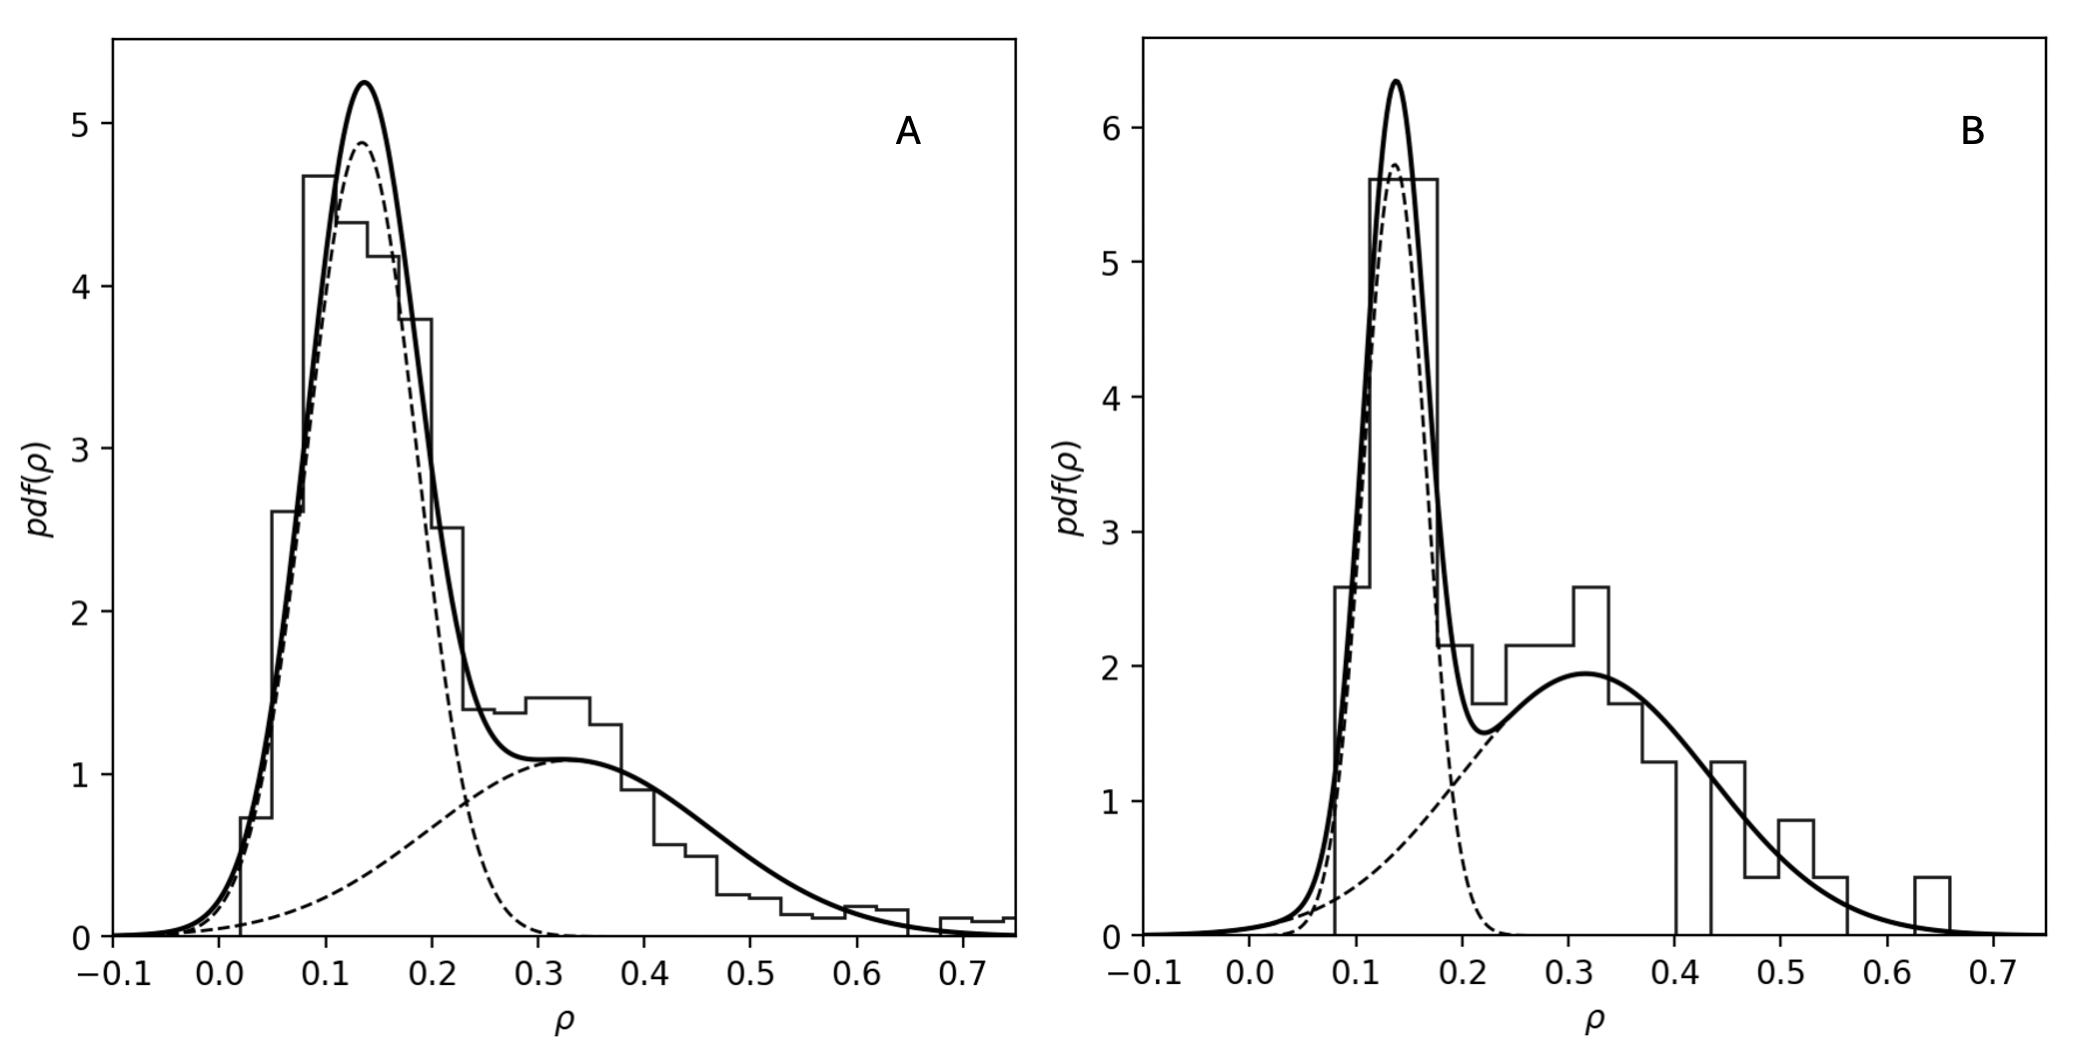
\includegraphics[width=1.0\linewidth]{Fig01f.png}
\caption{\label{fig:fig1} {\bf Figure title.} (A) MDPI ratio distribution for 2022 at the university level, Full line shows two-gaussian mixture fit, individual gaussians are plotted with dashed lines. (B) MDPI ratio distributions for 2022 at the country level.
}
\end{figure}

In figure 1 we show the MDPI ratio distribution with universities ranked in CWTS Leiden Open Ranking (panel A) for 2022. The distribution is well described by two-gaussian mixture $P(x) = \omega\mathcal{N}(x|\mu_1, \sigma_1) + (1-\omega)\mathcal{N}(x|\mu_2, \sigma_2)$ peaked around mean values $\mu_1, \mu_2$ for MDPI ratios with widths $\sigma_1, \sigma_2$. $\omega$ and $1-\omega$ are the weights of each gaussian peak in the mixture distribution. In panel B of Figure 1 we show the MDPI ratio distribution across countries with universities ranked in CWTS Leiden Open Ranking. The difference $\mu_2-mu_1$ in gaussian means is increasing with time between 2019 and 2023 as: 0.116, 0.186, 0.219, 0.196, 0.199, at the university level, and as: 0.086, 0.139, 0.174, 0.179, 0.232 at the country level. In both cases the separation between the two groups is increasing over time. 

\begin{figure}
    \centering
    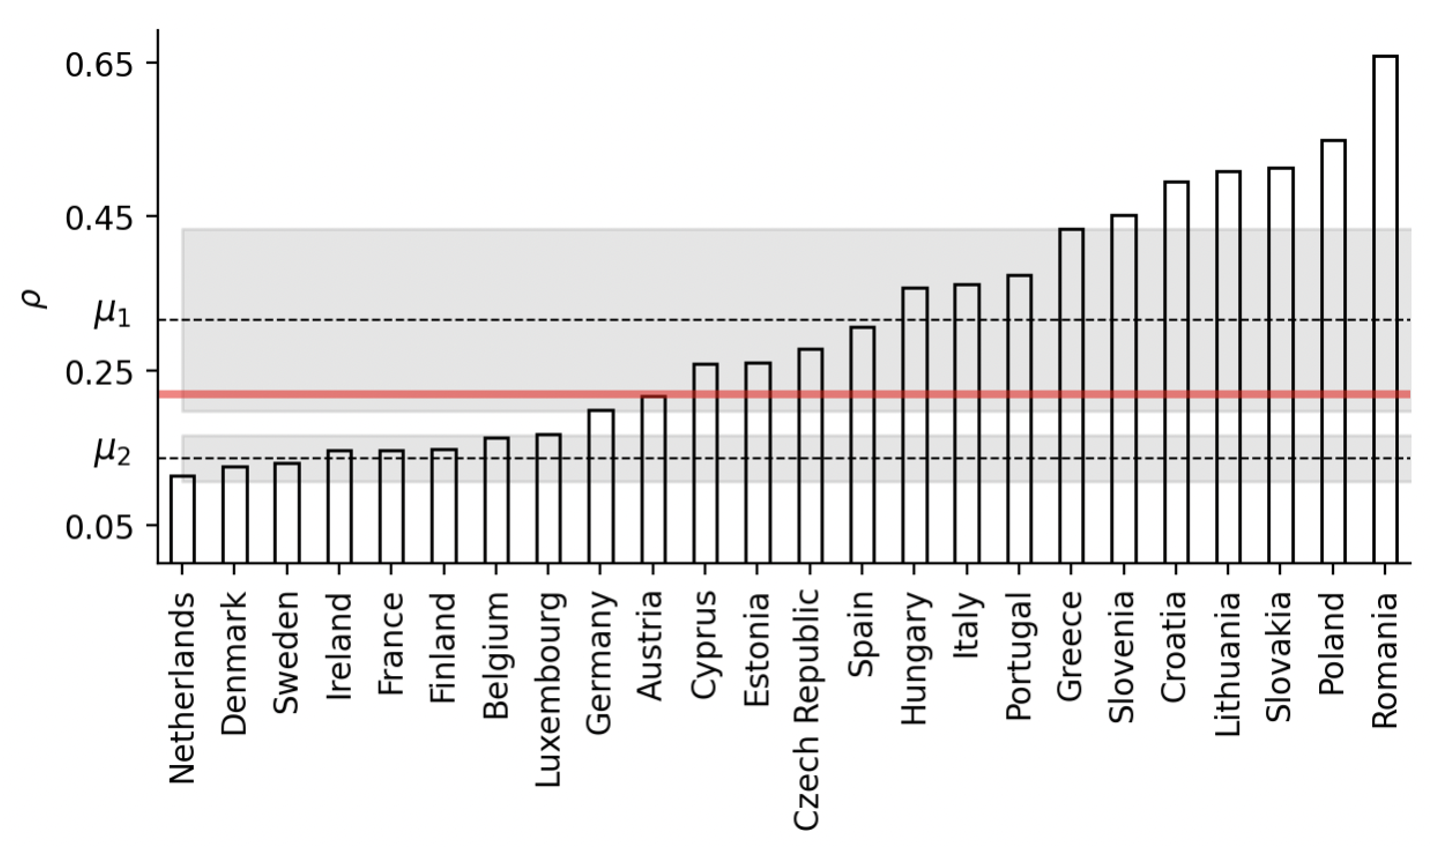
\includegraphics[width=1.0\linewidth]{Fig01af.png}
    \caption{\label{fig:fig2} {\bf Figure title.} MDPI ratio for 2022 for countries with universities ranked in CWTS Leiden Open Ranking. The thick horizontal line corresponds to the minimum of the two-gaussian mixture fit. The dotted lines are the means $\mu_1$ and $\mu_2$ of the two gaussians and the shaded bands are the widths $\sigma_1$ and $\sigma_2$.
    }
    \end{figure}

To see which countries comprise each of the two groups, we plotted the MDPI ratio for 2022 vs countries with universities ranked in CWTS Leiden Open Ranking in Figure 2. The thick horizontal line corresponds to minimum of the two-gaussian mixture fit and denotes the approximate separation of countries into two groups. The dotted lines are the means $\mu_1$ and $\mu_2$ of the mixed distribution model and the shaded bands are the corresponding standard deviations $\sigma_1$ and $\sigma_2$ of the two peaks. 

The data in Figure 2 indicates a clear separation of countries into two groups: $H_{MDPI}$, countries with a higher MDPI ratio moslty overlapping with the set of central and south-eastern EU countries (Croatia, Cyprus, Czech Republic, Estonia, Greece, Hungary, Italy, Lithuania, Poland, Portugal, Romania, Slovakia, Slovenia, Spain) and $L_{MDPI}$, countries with a lower MDPI ratio moslty overlapping with the set of central and north-western EU countries (Austria, Belgium, Denmark, Finland, France, Germany, Ireland, Luxembourg, Netherlands, Sweden). 

To see if the division of countries into $H_{MDPI}$ and $L_{MDPI}$ groups is statistically significant, we performed a Mann-Whitney U test. The test showed that the mean MDPI ratio for $H_{MDPI}$ countries is significantly higher than for $L_{MDPI}$ countries with $p<0.01$. Figure 3 displays the mean MDPI ratio separately for $H_{MDPI}$ and $L_{MDPI}$ countries. The gap and the increasing trend of the gap over the years in mean MDPI ratio between these two country groups is clearly visible. 

\begin{figure}
    \centering
    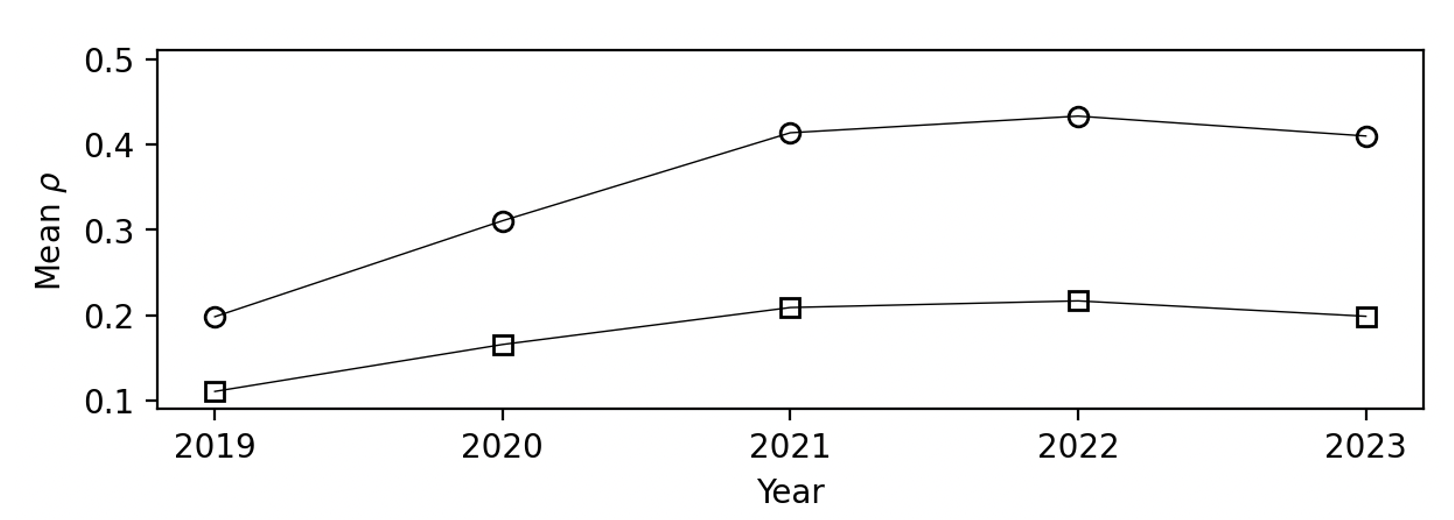
\includegraphics[width=1.0\linewidth]{Fig02f.png}
    \caption{\label{fig:fig3} {\bf Figure title.} Mean MDPI ratio vs years for $H_{MDPI}$ (open circles) and $L_{MDPI}$ (open squares) countries. Mann-Wittney U test shows statistically significant  differences in mean MDPI ratio between $H_{MDPI}$ and $L_{MDPI}$ countries with $p<0.01$.
    }
\end{figure}

\begin{figure}
    \centering
    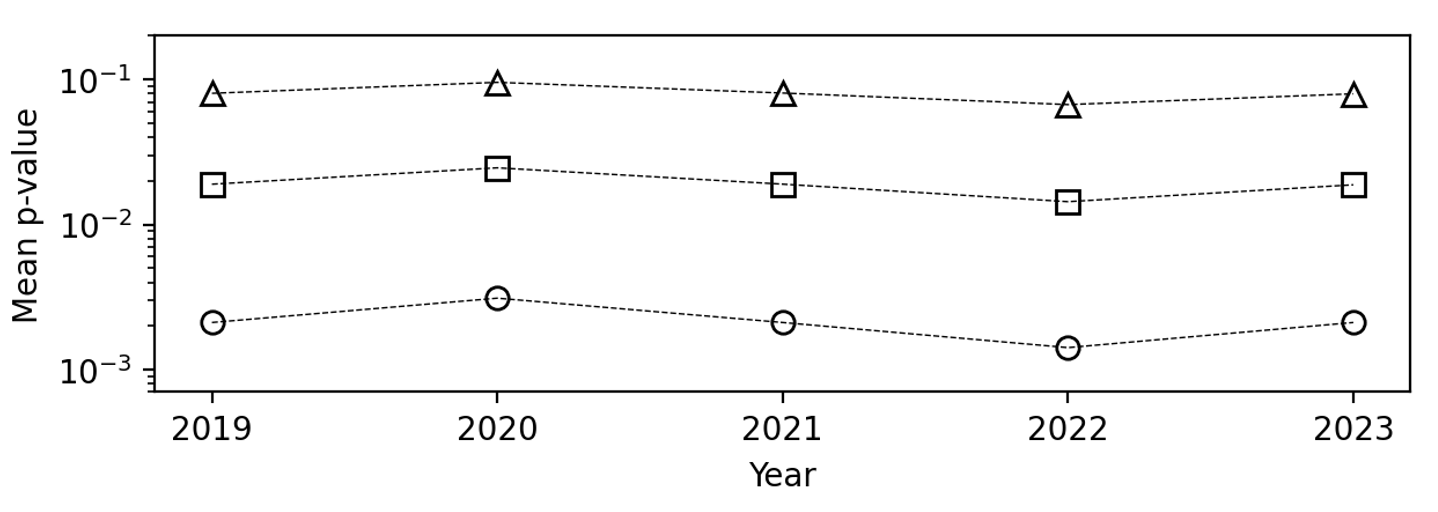
\includegraphics[width=1.0\linewidth]{Fig02af.png}
    \caption{\label{fig:fig4} {\bf Figure title.} Mean p-values for Mann-Whitney U test for differences in mean MDPI ratio between $H_{MDPI}$ and $L_{MDPI}$ countries. The p-values are calculated for 10000 random permutations of countries between the two groups in which 0 (open circles), 1 (open squares) or 2 (open triangles) countries are randomly switched between the two groups.
    }
\end{figure}

We also tested the robustness of the separation of countries into $H_{MDPI}$ and $L_{MDPI}$ groups by randomly switching countries between the two groups.
Figure 4 shows the mean p-values for the Mann-Whitney U test for the differences in mean MDPI ratio between $H_{MDPI}$ and $L_{MDPI}$ countries in which 0, 1 or 2 countries are randomly switched between the two groups. The p-values are calculated for 10000 such random permutations of countries between the two groups. The mean p-values vary very little between years for each permutation regime. When only one country is switched between the two groups the division between $H_{MDPI}$ and $L_{MDPI}$ countries is still statistically significant, however when switching two countries the division is no longer statistically significant showing the robustness of the separation of countries into $H_{MDPI}$ and $L_{MDPI}$ groups. 

\begin{figure}
    \centering
    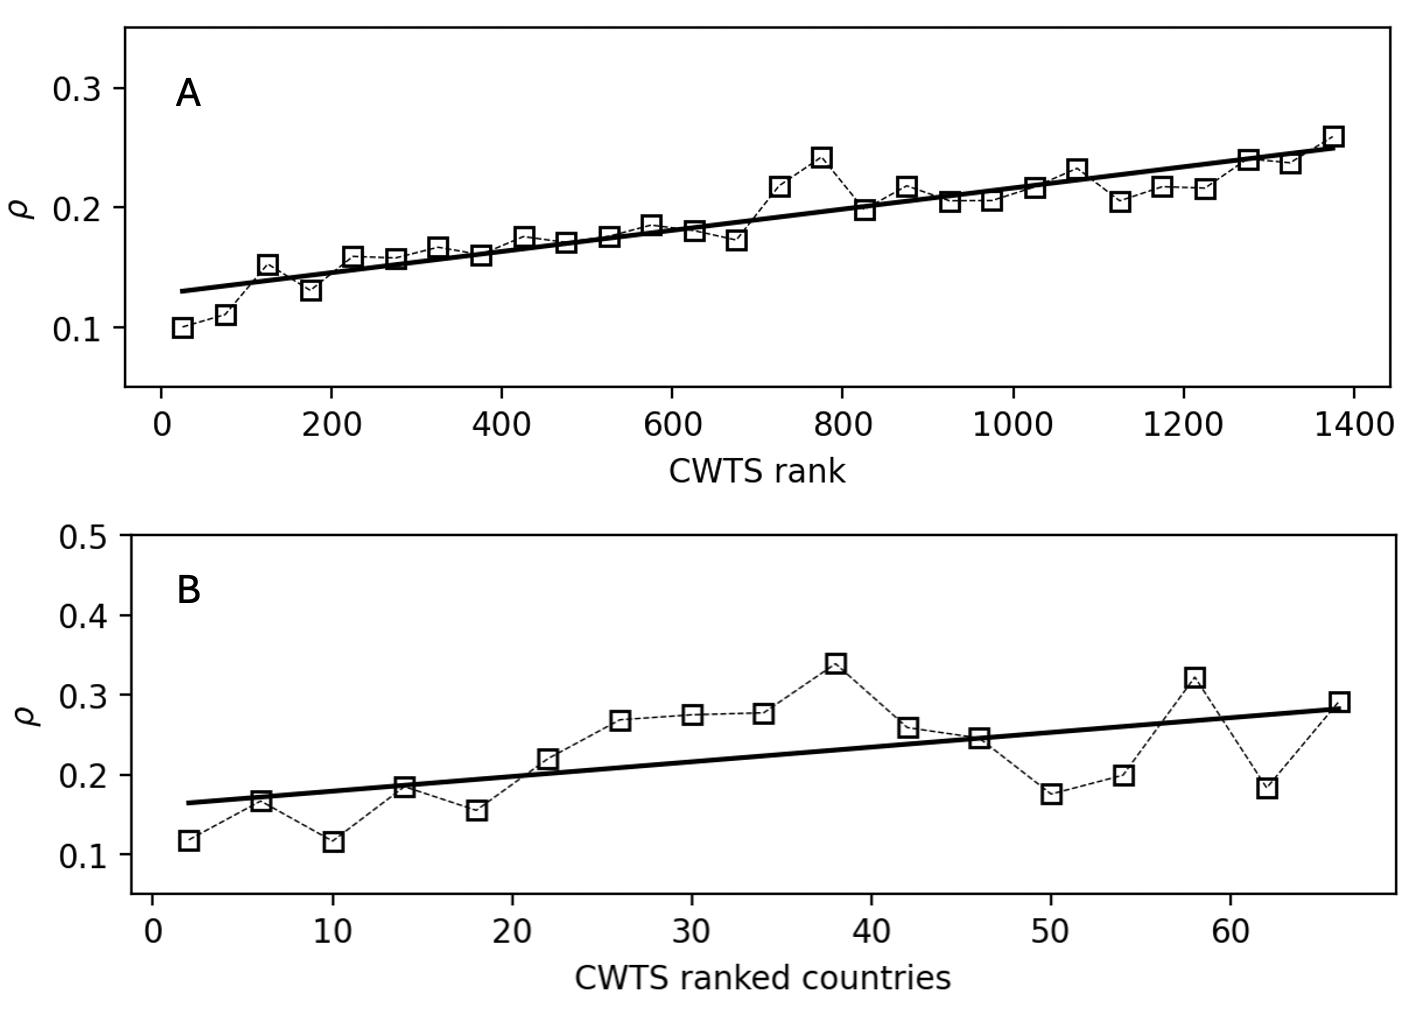
\includegraphics[width=1.0\linewidth]{Fig03f.png}
    \caption{\label{fig:fig5} {\bf Figure title.} 
}
\end{figure}

Research output measured through scholarly publications is one of key indicators in almost all university rankings so it should not be surprising that the scholarly publishing culture of universities might be closely related to their ranking. We checked this by comparing the MDPI ratio of universities with their rank in CWTS Leiden Open Ranking. In figure 5, panel A, we display the relationship between the MDPI ratio and the rank of universities included in CWTS Leiden Open Ranking table where the individual data points in the figure are the averages of MDPI ratios of universities in bins each 50 ranks wide. This relationship can be well described by a simple linear relationship between the rank of the university and its scholarly publishing culture. In panel B of figure 3 we show the relationship between the MDPI ratio and the rank of countries of universities included in CWTS Leiden Open Ranking table. 

\begin{figure}
    \centering
    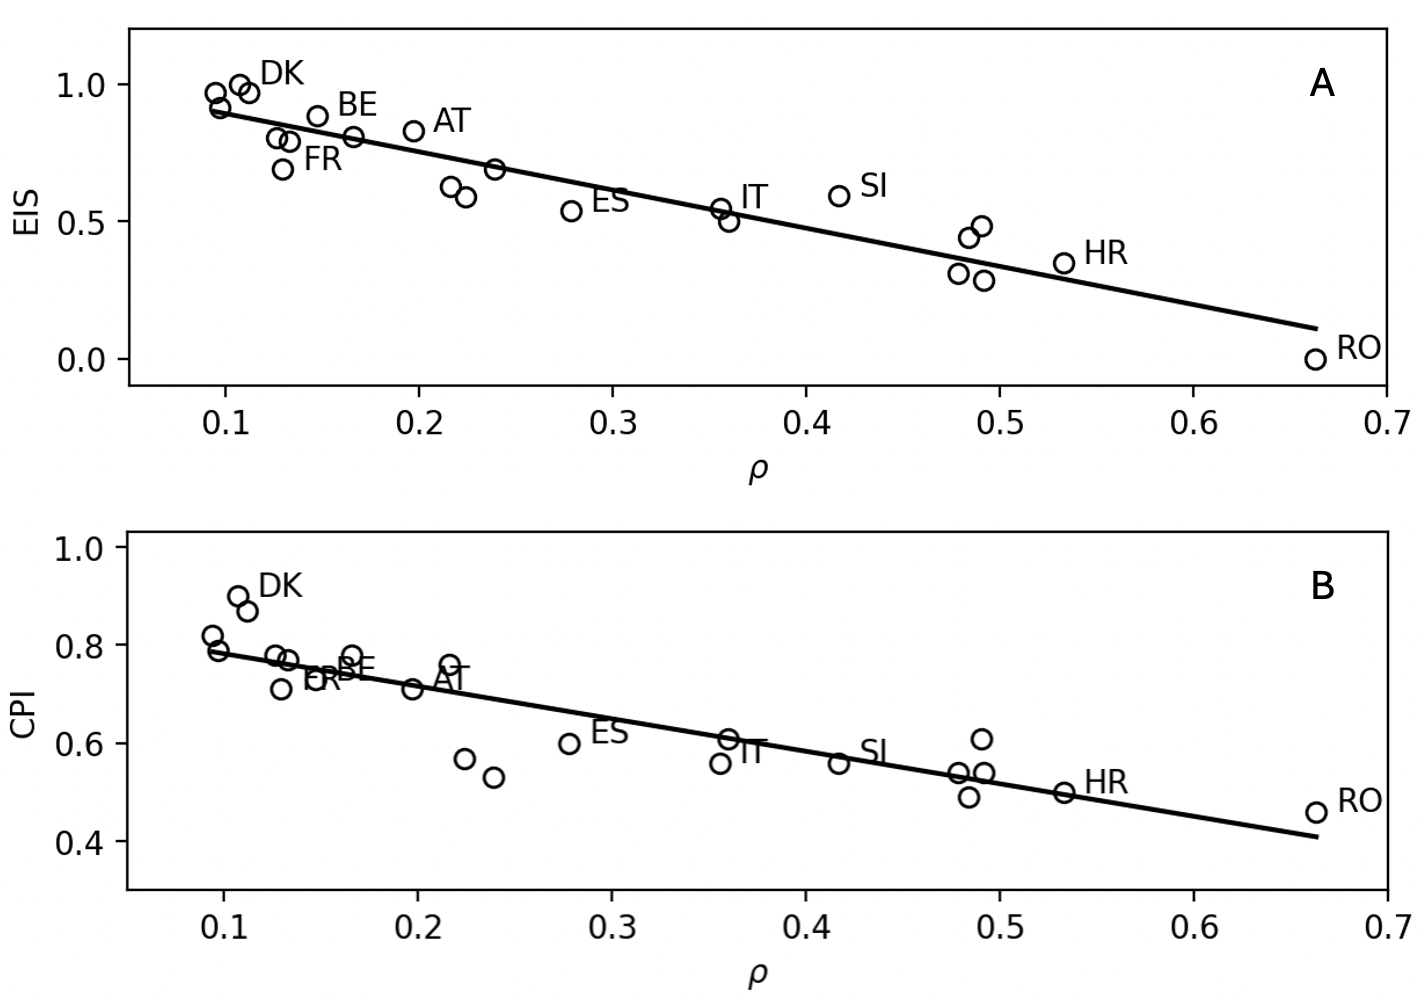
\includegraphics[width=1.0\linewidth]{Fig04f.png}
    \caption{\label{fig:fig6} {\bf Figure title.} Innovation potential, corruption perception and scholarly publishing culture
}
\end{figure}

Scholarly publishing culture of countries can also be related to their socio-economic context. Bringing together the data on innovation potential (European Innovation Scoreboard, EIS) and corruption perception (Corruption Perception Index, CPI) with the MDPI ratio of countries we can see how these factors are related to the scholarly publishing culture of countries. In figure 6 we show the relationship between the EIS (panel A), CPI (panel B) and MDPI ratio $\rho$ at a country level. For clarity only some of countries are indicated with country codes.
% correlation transitivity

\begin{figure}
    \centering
    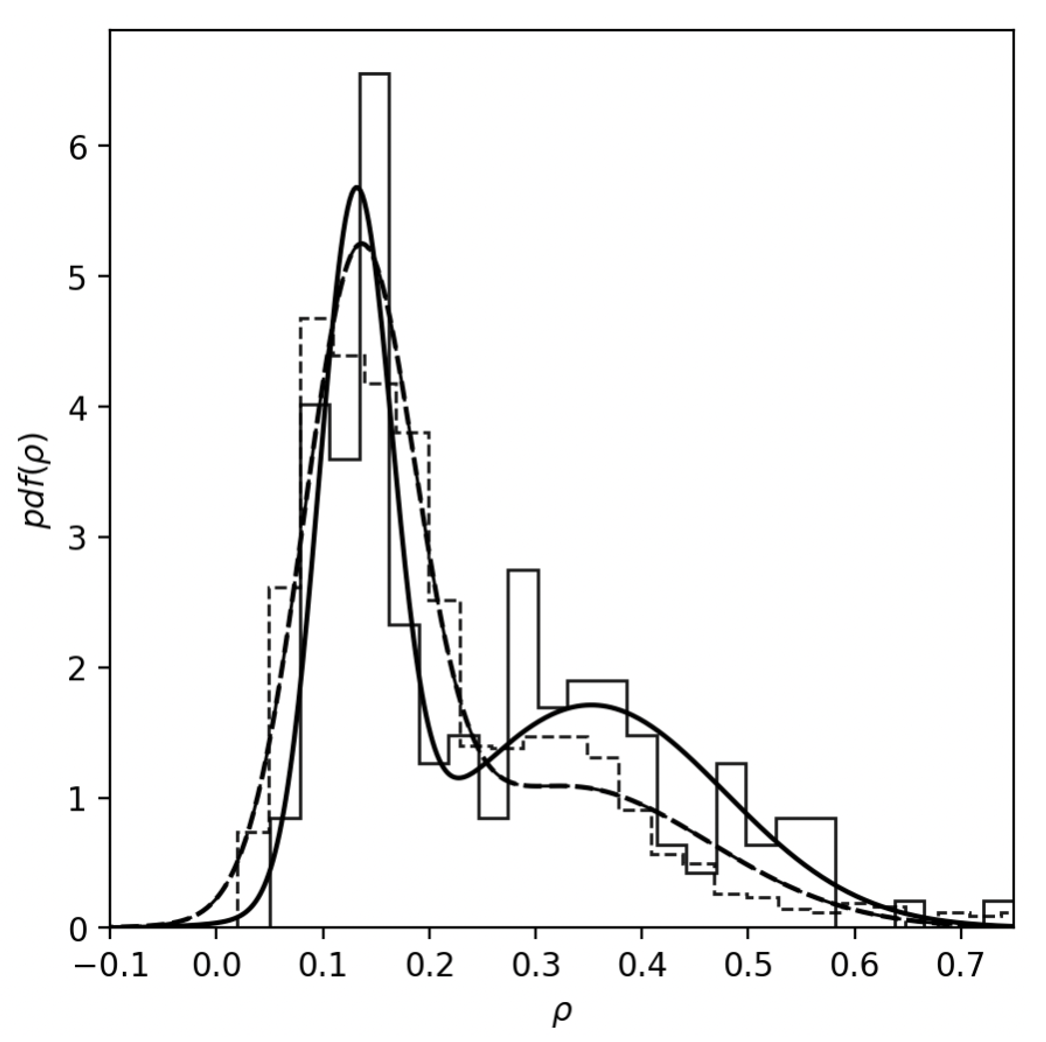
\includegraphics[width=.6\linewidth]{Fig05f.png}
    \caption{\label{fig:fig7} {\bf Figure title.} MDPI ratio distributions, CoARA universities  
}
\end{figure}

Figure 7 displays the distribution of MDPI ratio for CoARA universities included in CWTS ranking compared to all CWTS ranked universities. Both distributions are quite similar, exhibiting two-gaussian mixture shape. This puts CoARA group universities in a unique position where one can observe whether in the following years the shift towards more homogeneous publishing practice will happen driven by coalitions tenets.   

\section{Evolution of two cultures in scholarly publishing }
In one study~\cite{baccini2019citation} the authors examine how the introduction of bibliometric evaluations in Italy in 2011 led researchers to change their behavior, focusing more on self-citations and strategic citations to improve their evaluation scores. One way to understand such a shift is to use a game theoretical framework, where the new policy incentivizes researchers to prioritize self-promotion over traditional publication practices. This collective shift in behavior demonstrates how policy changes can significantly influence academic norms, leading to a new equilibrium where citation gaming becomes the dominant strategy to achieve career advancements. 

We showed that the MDPI ratio distribution in case of universities and countries is well described by two-gaussian mixed distribution which is a weighted sum of two gaussian distributions. Suppose that means and variances evolve with time much slower than the values of the weight $\omega\in [0, 1]$.  Therefore, the shape of $P(x)$ will be mostly determined by the time evolution of $\omega$. The emergence of two cultures in scholarly publishing when $\omega > 0$ or when the second peak with $\mu_2 >\mu_1$ occurs.  

To show how two distinct cultures can emerge from a single culture within the realm of scholarly publishing in the EU, we use a game theory approach. The game involves researchers choosing between two strategies: publishing in established, legacy journals with typically slow reviewing processes (strategy B) or in new, fast-reviewing, open-access journals (strategy A). Initially, most researchers follow strategy B, reflecting the traditional approach. However, an increasing push for open science and the appeal of rapid dissemination create incentives for adopting strategy A. 

\begin{equation}
    u_1 = P(e_1, e_2)R - e_1
\end{equation}

\begin{figure}
    \centering
    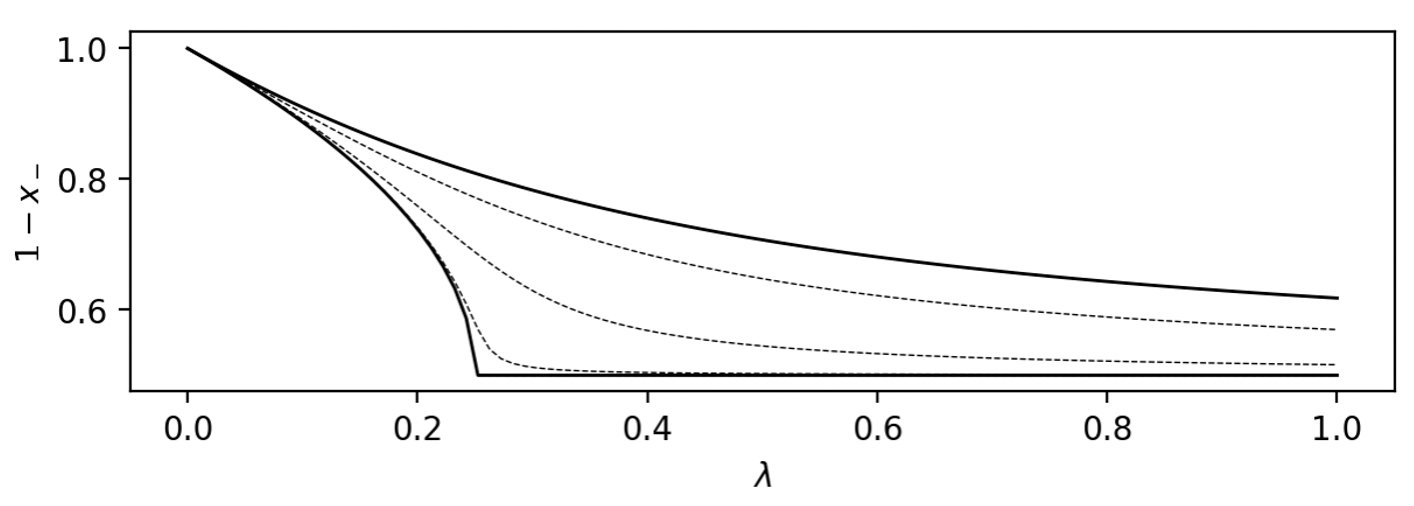
\includegraphics[width=1.0\linewidth]{Fig07.png}
    \caption{\label{fig:fig7} {\bf Figure title.} Game theory model of scholarly publishing culture evolution. Researchers choose between two strategies: publishing in established, legacy journals with typically slow reviewing processes (strategy B) or in new, fast-reviewing, open-access journals (strategy A). 
}
\end{figure}

Researchers payoffs depend on coordination with peers; citation practices, visibility, academic recognition-prestige, cost, speed  




\section{Discussion}
Our findings reveal significant insights into the current state and evolving trends of scholarly publishing practices among universities and EU countries. Using open research information of scholarly publications and university ranking we showed that there is a clear bifurcation in publishing cultures in Europe. 

The separation, evident at both the university and country levels, indicates a growing divergence in publication strategies, influenced by factors such as policy changes and institutional rankings. The increasing gap between $H_{MDPI}$ and $L_{MDPI}$ countries underscores the impact of regional dynamics on academic publishing. Additionally, the correlation between publishing practices and factors like innovation potential and corruption perception suggests that broader socio-economic contexts play a role in shaping research outputs. 

The tendency of researchers from $H_{MDPI}$ countries and lower-ranked institutions to publish more in open-access MDPI journals, which provide faster turnaround and are often perceived as less stringent, may be explained in several ways. As publishing behavior is generally the result of a reasoned process, our findings can be interpreted through the lens of the Theory of Planned Behavior~\cite{ajzen1991}, which recognizes the critical role of individuals ability (i.e., perceived behavioral control) and motivation (i.e., intentions, which are heavily influenced by subjective norms and attitudes). While this theory has not yet been studied in the context of explaining researchers’ decision to publish in MDPI over more traditional journals, Moksness and colleagues~\cite{moksness2020} have used it to explain intentions to publish in open-access journals.

First, in relation to perceived behavioral control, researchers from $H_{MDPI}$ and lower-ranked countries may perceive important internal and external barriers to publishing in traditional, legacy journals, such as resource constraints (including financial aspects), fewer international collaboration opportunities, language barriers, and less prestigious institutional affiliations. In fact, recent research suggests that some of these barriers objectively exist; for example, a recent study by Sverdlichenko and colleagues~\cite{sverdlichenko2022} revealed that journal editors may be influenced by author institutional affiliations when deciding whether a manuscript should be sent out for peer review. Second, regarding subjective norms, academics working in $H_{MDPI}$ and lower-ranked countries may feel a stronger social pressure to publish frequently, potentially driven by institutional policies that still reward the quantity (instead of quality) of publications. This may lead to a snowball effect, with early adopters of such practices imposing pressure on others to do the same to remain competitive in their academic environment. Over time, publishing in MDPI over legacy journals can become completely normalized or even desirable in certain academic environments. The important role of social norms, as opposed to solely top-down regulations, in determining researchers publication choices has been previously discussed by other authors (e.g., Migheli and Ramello~\cite{migheli2013}). Lastly, several aspects may contribute to more favorable attitudes towards MDPI in $H_{MDPI}$ and lower-ranked countries. For example, they may believe that publishing in MDPI will help them achieve their academic goals, such as career advancement, quicker, or increase their visibility (due to the open-access nature of these journals).

We also found that researchers from countries with higher corruption perception are more likely to publish in MDPI over the Big Five journals. While this relationship has not yet been investigated in other countries, some parallels can be drawn from the broader literature on the characteristics of individuals who live in countries perceived as highly corrupt. For example, it is well-known that perceptions of corruption are associated with lower institutional trust~\cite{hakhverdian2012}, lower meritocratic ideology~\cite{tan2017}, and adaptive behaviors, whereby societal levels of corruption result in norm and rule violations on the individual level~\cite{kobis2018}. In the specific context of scholarly publishing, researchers may distrust the fairness of the peer-review processes and traditional publishing practices and merits in general. Moreover, environments with high corruption may sometimes be characterized by uncertain career advancement procedures and less transparent and equitable funding, motivating researchers to publish quickly to bolster their CVs and improve their chances in these ambiguous circumstances. 

Our findings raise concerns about the potential inequalities in scholarly publishing across Europe. The preference for MDPI publications in $H_{MDPI}$ countries and lower-ranked universities may be influenced by factors such as publication speed and perceived ease of acceptance but could also indicate various challenges faced by researchers in these environments, such as fewer resources available for research and systemic issues that push researchers towards certain publication outlets. In line with this, governments and institutions in $H_{MDPI}$ countries should continue enhancing their support for research activities (e.g., transparent funding procedures, budgets for article processing charges) and empowering academics with better infrastructure, mentoring, and collaboration options. Moreover, extensive efforts should be dedicated to promoting transparent and fair evaluation metrics that go beyond the mere quantity of publications. 

mutations: incentives, funding, legislation, open access, APCs, prestige, career advancement, research quality, collaboration, citation practices, visibility, academic recognition, innovation potential, corruption perception, socio-economic contexts, regional dynamics, policy changes, institutional rankings,
Labor law, universities and research assessment systems across EU: north-west vs south-east comparison 
Response of countries to open access/science EU initiative and the NW-SE divide... $H_{MDPI}$ vs $L_{MDPI}$ gap, ERA harmonization
  
\begin{center}
--\,--\,--\,--\,--
\end{center}
\vspace{1mm}
\noindent\textbf{Acknowledgements.} DK received financial support from the Slovenian Research Agency (the research core funding program P3-0396 and the research project no.J7-3156). 

\noindent\textbf{Code and data availability.} The data and the code used in this work is available at \url{https://github.com/deankorosak/two-cultures/}.

\noindent\textbf{Author contributions.} All authors contributed substantially to all aspects of the study.

\noindent\textbf{Conflict of interest.} The authors declare no conflict of interest, financial or otherwise.
 

\bibliography{refs}{}
\bibliographystyle{apsrev4-1}

\end{document}